% Chapter Template
\part{Physics introduction}
\chapter{The Standard Model and Beyond} \label{Chapter1} 

\section{Introduction}
Starting from late 19th century and progressing in the first half of the 20th century, 
the theories and discoveries of thousands of physicists have led to a significant insight into the fundamental structure of matter. 
By the 1960s, physicists had promote quite a collection of what they assumed to be fundamental particles, basic building blocks of matter that could not be resolved any further into sub-pieces. 

In 1964, theorists Murray Gell-Mann~\cite{GELLMANN1964214} and George Zweig~\cite{Zweig:570209} theorized that many components of the so-called ``particle zoo'' were composite particles consisted of even smaller parts, which are now called quarks. The list of fundamental particles was further reduced, the description of the fundamental forces which govern the interaction between them was added and new patterns were begun to appear. This was the outset of the development of the Standard Model of particle physics.
The first references to the so-called “standard model” can be found in papers published in the 1970s~\cite{Pais:1975gn,PhysRevD.13.680} and only in the '80s and '90s the \emph{S} and \emph{M} got capitalized.

To this day, the Standard Model (SM) has successfully interpreted nearly all experimental results and accurately predicted a wide variety of phenomena getting even more credits with the latest foreseen discoveries such as top quark observation (1995) and Higgs boson discovery (2012). Even though it is considered the most solid description of the subatomic world, we see some holes when trying to address the full picture.\\
Those unexplained aspects, which are going to be specified in Sec.~\ref{sec:bsm}, have inspired the big hunt for new physics that has drawn the creation of so many new experiments and that has fed fresh exotic theories. This thesis cooperates in this attempt.


\section{The Standard Model of Elementary Particles}\label{sec:sm}
Figure~\ref{fig:SMfig} shows the building blocks of the Standard Model, either they are matter particles, everyday matter
or exotic matter created in particle accelerators and in the early universe, or they are the additional force-carrier particles.

In the Standard Model, the elementary particles are grouped into two main categories on the basis of the statistic they obey and consequently of the spin: fermions and bosons. 
\begin{figure}[h]
\centering
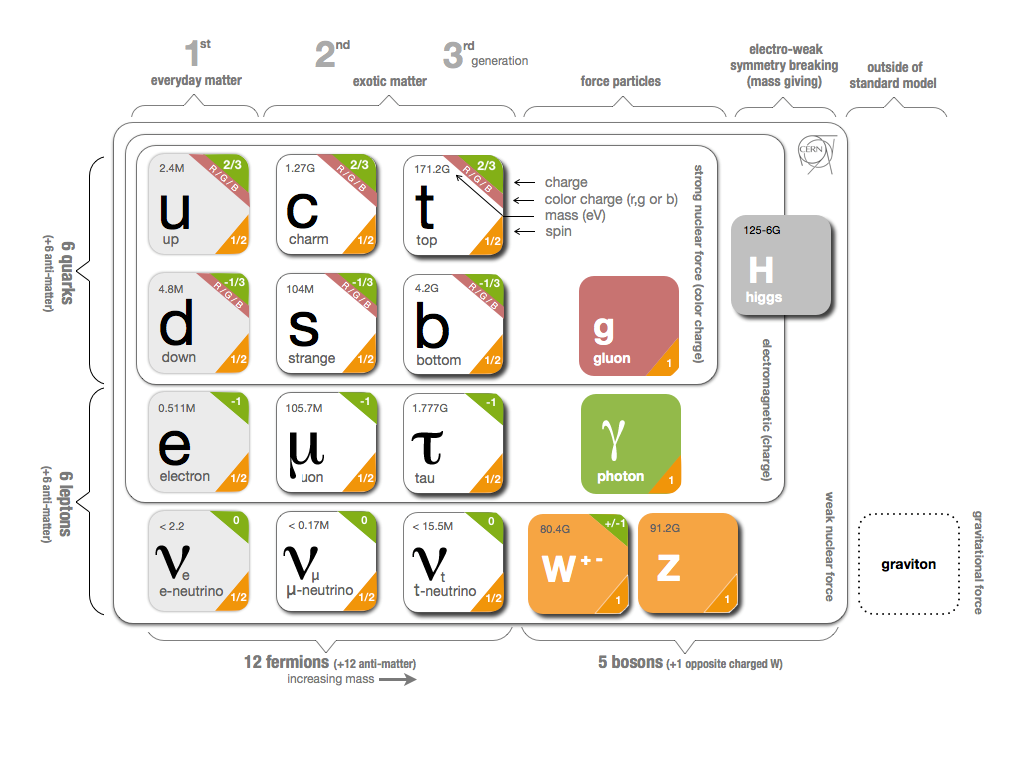
\includegraphics[clip,trim=1cm 2cm 2cm 1cm, width=0.75\textwidth]{Figures/c1/SMinfographic_image.png}
\caption{Elementary particles of the Standard Model (infographic
  developed for~\cite{particlefest})}
\label{fig:SMfig}
\end{figure}

The fermions are particles which follow the Fermi-Dirac statistic and correspondingly have half odd integer spin (1/2, 3/2, 5/2...). They do obey the Pauli exclusion principle and therefore they have different symmetry properties, with respect to bosons, when exchanging of two identical particles: the total wave function of a system of two identical fermions is antisymmetric for fermions. This lead to the fact that, in a rigorous way, if two identical (in spin and space coordinates) fermions interchange the total wave function changes its sign. Thus, two or more identical fermions can not simultaneously exist in the same quantum state. On the contrary particles with an integer spin like the bosons which follow the Bose-Einstein statistic do not obey the Pauli exclusion principle and can occupy the same quantum state. 

In the Standard Model, there are two types of elementary fermions: quarks (which form hadrons such as protons and neutrons) and leptons. 
Moreover, the fermions are grouped in three generations and each generation has two types of leptons and two quarks. The two leptons have one electric charge -1, the other one is neutral; the two quarks have charges $-1/3$ (down-type) and $+2/3$ (up-type). Between generations electric and strong interactions are identical while particles differ by their flavor quantum number and mass.  The first generation consists of electrons ($e$) and electron neutrinos ($\nu_e$) and of quarks \emph{up} and \emph{down}. All the everyday matter is composed by up-down quarks and electrons. The second generation is made of muons ($\mu$) and muon neutrinos ($\nu_\mu$) and of quarks \emph{charm} and \emph{strange}. The third generation is composed by taus ($\tau$) and tau neutrino ($\nu_\tau$) and by quarks \emph{top} and \emph{bottom}. The particles of higher generation have larger masses than the preceding one, this has the effect that leptons and quarks of the second and third families are more unstable with shorter life-time and can easily decay back to elements from the first generation.\\
Each of the 12 fermions has an anti-matter particle which presents all the charges reversed.

The fermions, just described, interact exchanging the bosons particles. The elementary bosons are force carriers and each of them is associated to a fundamental force. The photon ($\gamma$) is the mediator of the electromagnetic force, it has spin equal to 1, it is neutral and massless. The $\PW^{\pm}$ and \PZ are mediators of the weak force, they have spin 1, the $\PW^{\pm}$ have unitary charge (+1 or -1) while \PZ is neutral; the are heavy in mass ($M_\PW =\:$80.379 $\pm$ 0.012\GeV~\cite{pdgw}, $M_\PZ =\:$91.1876 $\pm$ 0.0021\GeV~\cite{pdgz}) and very short-lived. The quarks possess color charge which means they are subject to the strong interaction mediated by the gluons ($g$) which likewise are associated to a color charge. For a property of the strong interaction known as color confinement, quarks can not exist isolated. Thereupon quarks and gluons must cluster together to for hadrons which are color neutral (white) and which can exist and propagate freely. The hadrons can be made of either a quark and anti-quark, \emph{mesons} or three quarks, \emph{baryons}. The mesons are composite bosons (spin 0 or 1) while baryons are composite fermions. Quarks, besides interacting through strong force, could also transform into quarks of another flavor through weak interaction by absorbing/emitting a \PW boson. The strengths/probabilities of the weak interactions between the six quarks do not have all the same magnitude (some are more preferable) and they are described by the values in the Cabibbo–Kobayashi–Maskawa matrix~\cite{10.1143/PTP.28.870}.\\
The massive bosons get their mass thanks to the interaction with the quantum field. The so-called Brout–Englert–Higgs (BEH) mechanism refers to the generation of masses for the three weak gauge bosons (\PW, \PZ) through electroweak symmetry breaking~\cite{PhysRevLett.13.321,PhysRevLett.13.508}. The mathematical treatment of Standard Model and of the BEH mechanism is presented in Sec.\ref{sec:mathSM}.\\
The last fundamental force, gravity, is not included in the Standard Model framework. 

The leptons are not affected by the strong interaction while they are subject to electromagnetic and weak interactions. As already said, the six leptons are organized in three generations, then are arranged in three left-handed weak isospin doublets where charged and neutral leptons share the same left-handed helicity. Each doublet has a different lepton number which has to be conserved during all the interactions implying that leptons and anti-leptons must be created in pairs of a single generation. The only violation of this universal lepton number conservation can be observed in weak interaction in the neutrino oscillations where is there a transformation between different generations. The neutrino oscillation and the obvious consequences are going to be extensively explained in Sec.~\ref{sec:bsm}. 


\section{The mathematical formulation of the Standard Model}\label{sec:mathSM}
This section describes the mathematical framework of the Standard Model of particle physics, which is a gauge Quantum Field Theory (\emph{QFT}). For an extensive discussion and explanation of QFT and of the Standard Model refer to~\cite{Bardin:1999ak}.
\subsection{Quantum Field Theory and Gauge invariance}\label{sec:qft}
In a QFT theory, the fundamental objects are described as quantum fields with specific transformation properties governed by a set of symmetry groups. The fields are: the \emph{fermion} fields $\psi$, the \emph{electroweak boson} fields $W_1, \; W_2, \; W_3,$ and $B$, the \emph{gluon} field $G_a$ and the Higgs field $\phi$. The dynamics of those quantum fields are completely determined by the Lagrangian density, $\mathcal{L}$. \\
The description of QFT starts with a Lagrangian density $\mathcal{L}$, a function of the fields in the system and their derivatives, and possibly the space-time coordinates; minimizing the action ($\mathcal{S}$), which is the space-time integral of $\mathcal{L}$, the equation of motion can be extracted:
\begin{equation}
\label{eq:action}
 \mathcal{S} \;\; = \;\; \int \mathcal{L}(x) \ d^4x,
\end{equation}
where x is the space-time coordinate.

The complete Standard Model Lagrangian contains specific terms for every one of the fundamental interactions. In the rest of the section all these elements and the corresponding meanings are going to be illustrated and clarified.

To start, consider the Lagrangian of a free spinor field $\psi$ which contains a kinetic and mass term:
\begin{equation}
\label{eq:dirac}
 \mathcal{L}_{Dirac} \;\; = \;\; \overline{\psi}(x)\ (i\gamma^{\mu}\partial_{\mu} - m ) \psi(x)
\end{equation}
where the Einstein notation is used which implies summation over the indices $\mu \in 0,1,2,3$; $m$ is the fermion's mass, $\gamma^{\mu}$ are the gamma matrices ($\gamma^{\mu}\gamma^{\nu} + \gamma^{\nu}\gamma^{\mu} = 2g^{\mu\nu}$ with $2g^{\mu\nu}$ is the Minkowski metric) and $\partial_{\mu}$ is the space-time derivative $(\nicefrac{\partial}{\partial_{t}}, \nicefrac{\partial}{\partial_{x}}, \nicefrac{\partial}{\partial_{y}}, \nicefrac{\partial}{\partial_{z}})$. The $\psi(x)$ denotes the Dirac fermion field and the anti-fermion field, the adjoint spinor $\overline{\psi}(x)$ is defined as $\psi^\dag\gamma^{0}$, with $\psi^\dag$ the hermitian conjugate of $\psi$.

The QFT is gauge theory which means it is based on the hypothesis that some symmetries, \ie transformations that leave the Lagrangian of the system unchanged, are possible not only globally, but also locally.
Most theories of physics are described by Lagrangians who are invariant under certain transformations of the coordinate system performed simultaneously at every point in spacetime: they are therefore said to have global symmetries. A local symmetry is one that keeps a property invariant when a possibly different symmetry transformation is applied at each point of spacetime; specifically a local symmetry transformation is parameterized by the spacetime co-ordinates, whereas a global symmetry is not. The concept underlying gauge theories is precisely to postulate that Lagrangians must also possess local symmetries, i.e. gauge symmetries and gauge invariant.\\
Going back to Eq.~\ref{eq:dirac}, this Lagrangian is invariant under a global U(1) phase transformation
\begin{equation}
\label{eq:globalT}
 \psi(x) \rightarrow \psi'(x) = e^{-i\omega} \psi(x), \; \; \; \; \; \;    \overline{\psi}(x) \rightarrow \overline{\psi'}(x) = e^{i\omega} \overline{\psi}(x),
\end{equation}
with $\omega$ is a constant. Thus, the requirement is for this Lagrangian to be invariant under a local U(1) transformation
\begin{equation}
\label{eq:localT}
 \psi(x) \rightarrow \psi'(x) = e^{-i\omega(x)} \psi(x), \; \; \; \; \; \;    \overline{\psi}(x) \rightarrow \overline{\psi'}(x) = e^{i\omega(x)} \overline{\psi}(x),
\end{equation}
where now $\omega(x)$ is a function of the spacetime point $x$. Considering then that $\partial_{\mu}$ would also act on $\omega(x)$, to make the 
Lagrangian invariant under this gauge symmetry, a new term, vector field, $A_{\mu}$ has to be introduced in Eq.~\ref{eq:dirac}:
\begin{equation}
\label{eq:GS1}
 \mathcal{L}_{Dirac} \;\; = \;\; \overline{\psi} (i\gamma^{\mu} (\partial_{\mu} + igA_{\mu})-m) \psi \;\;\; \equiv  \;\;\; \overline{\psi} (i\gamma^{\mu}\mathcal{D}_{\mu}-m) \psi 
\end{equation}
(the $(x)$ dependence is omitted from the notation)\\ $A_{\mu}$ is the gauge field which couples to the spinor field $\psi$ with a coupling strength $g$; $\mathcal{D}_{\mu}$ is called covariant derivate and it is defined as $\mathcal{D}_{\mu} = \partial_{\mu} + igA_{\mu}$. \\
The $\mathcal{L}_{Dirac}$ in Eq.~\ref{eq:GS1} is invariant under local trasformation ($\mathcal{L}_{\psi} =\mathcal{L}_{\psi'}$) requiring:
\begin{equation}
\label{eq:GS2}
A_{\mu} \rightarrow A'_{\mu} =  A_{\mu} + \frac{1}{g}[\partial_{\mu} \omega(x)]
\end{equation}

This example has made it clear that asking the Lagrangian to be gauge invariant under a certain gauge transformation, gauge fields are naturally introduced in the $\mathcal{L}$ itself. These fields entail the existence of the gauge bosons, spin 1 particles, which couple to the fermions. \\
Defining the field strength tensor $F_{\mu\nu} = \partial_{\mu}A_{\nu} - \partial_{\nu}A_{\mu}$\footnote{The field strength tensor is defined as $F^{a}_{\mu\nu} = \partial_{\mu}A^{a}_{\nu} - \partial_{\nu}A^{a}_{\mu} + g f^{abc} A^{b}_{\mu}A^{c}_{\nu}$ for the gauge field $A_{\mu}$ with gauge constant $g$. The structure constant $ f^{abc}$ vanish since U(1), here used, in an Abelian commutative group.}
, the final gauge invariant $\mathcal{L}_{Dirac}$ can be written as
\begin{equation}
\label{eq:GS3}
 \mathcal{L}_{Dirac} \;\; = \;\; -\frac{1}{4} F_{\mu\nu} F^{\mu\nu} + \overline{\psi} (i\gamma^{\mu} (\partial_{\mu} + igA_{\mu})-m) \psi \;\;\;\;\;\; \footnote{In this equation the mass term is not invariant under local transformation. The boson they remain massless up to this point, the concept of spontaneous symmetry breaking is going to be introduced later in Sec~\ref{sec:symBreaking}}
\end{equation}

\vspace{10mm}
The example here was carried out for a U(1) unitary transformation which can be described by one, $n^2$ degree of freedom (or generator of the gauge group U(1)). U(1) is an Abelian commutative group.  \\
As preface for the next section the general case for a special unitary group of order \emph{n}, SU(\emph{n}), is presented here. The special unitary group SU(\emph{n}) is the Lie group of  $n\times n$ matrices with determinant 1. The group is described by a set of $n^2 -1$ gauge generators, $T^a$ with $a \in (1, 2, ... , n^2 -1)$. The covariant derivate of SU(\emph{n}) is then $\mathcal{D}_{\mu} = \partial_{\mu} + igT^aA^a_{\mu}$ and it corresponds to an $n\times n$ matrix. At the same time, there are $n^2 -1$ gauge bosons which construct the currents and mediate the interaction.\\
The gauge group can be Abelian, like U(1), or non-Abelian; the latter case means that the generators of the group do not commute. At a different level, it means the field strength tensor and the kinetic term for the gauge fields in the Lagrangian naturally allows for
self–interactions of the gauge bosons. A theory with a local non-Abelian phase transformation is called a Yang-Mills theory.


\subsection{The Standard Model gauge group}\label{sec:gauge group}
Three symmetries are intensified to be necessary and sufficient in the SM theory to address and describe the experimental results of the particles and of their interactions. The Standard Model is described by $SU(3)$ $\otimes$ $SU(2)$ $\otimes$ $U(1)$ gauge symmetry group; each subgroup has the corresponded gauge field.\\
As it was explained in the previous section, the SM Lagrangian manifests a $U(1)$ local phase invariance. The associated gauge field to this Abelian invariance of the theory is called $B_\mu$. There is then the second invariance, under non-Abelian transformations that build an $SU(2)$ group, which introduces three $W^i_\mu$ fields ($i = 1,2,3$), one for each of the three generators of $SU(2)$. The last invariance non-Abelian that forms $SU(3)$ leads to the introduction of eight $G^a_\mu$ fields ($a = 1,...,8$).\\
The covariant derivative which guarantees the full SM Lagrangian invariant under the three transformation described above is:
\begin{equation}
\label{eq:SMderivative}
\mathcal{D}_{\mu} \;\; = \;\; \partial_{\mu} + ig_1\frac{Y}{2}B_{\mu} - ig_2\frac{\sigma^i}{2}W^i_{\mu} - ig_s\frac{\lambda^a}{2}G^as_{\mu}
\end{equation}
where $Y$, $\sigma^i$ and $\lambda^a$ represent the generators for the $U(1)$ weak hypercharge, the $SU(2)$ weak isospin and the $SU(3)$ color space, respectively. The $SU(2)$ generators in the third term of Eq.~\ref{eq:SMderivative} are the $2\times2$ Pauli-matrices $\sigma^i$ and the $SU(3)$ generators, the forth term in ~\ref{eq:SMderivative}, are the $3\times3$ Gell-Man matrices $\lambda^a$ ($a = 1,...,8$).\\

In the following sections the distinct terms in the full SM Lagrange are introduced and explained. Starting from the $\mathcal{L}_{Dirac}$ in Eq.~\ref{eq:GS1} and using the covariant derivative of Eq.~\ref{eq:SMderivative}, the SM Lagrangian becomes then invariant under the three gauge groups transformations describing the fermions behaviors under the gauge transformations and their interactions among all the particles of the SM. To fully illustrate the way fermions operate under the gauge transformations it is fundamental to quantify the charge fermions bring with respect to the gauge interaction. Those charges have to be determinated from experimental results and they can not be anticipated by the theory.

\subsubsection{The Electroweak theory}\label{sec:ewk}
The Electroweak theory gives an unified description of the electromagnetic and the weak forces, by asking gauge invariance under the $SU(2)_{L}$ $\otimes$ $U(1)_{Y}$ gauge symmetry group, whit the subscript $L$ referring to the left-handed chiral structure of $SU(2)$.\\
Introducing the chiral projection operators:
\begin{equation}
\label{eq:LRoperators}
P_L=\frac{1}{2} (1-\gamma^5), \;\;\;\ P_R=\frac{1}{2} (1+\gamma^5), \;\; \;\; \;\; (\text{defing} \;\; \gamma^5 = i\gamma^0\gamma^1\gamma^2\gamma^3)
\end{equation}
the Dirac spinors $\psi$ can be projected onto the right-handed (RH) chiral states and the left-handed (LH) chiral states as:
\begin{equation}
\label{eq:LR1}
\psi = \begin{pmatrix}
\psi_L\\
\psi_R
\end{pmatrix}
\end{equation}
with $\psi_L$, $\psi_R$ as left- and right-handed Weyl spinors. Replacing the spinor in the Lagrangian, massless fermions are decoupled into LH and RH particles:
\begin{equation}
\label{eq:LR2}
\overline{\psi} \gamma^{\mu} \psi \;\; = \;\; \overline{\psi}_L\gamma^{\mu} \psi_L +  \overline{\psi}_R\gamma^{\mu} \psi_R
\end{equation}
where, for massless fermions, their chirality coincides with their helicity. Sustained by clear experimental results for the parity-violating nature of the ElectroWeak theory, the weak-isospin charge appears to be different for particles with different chirality and it looks that the corresponfing gauge fields interact only with LH fields. Thus the LH fermions fields are grouped in doublets, for example ($e_L,\nu_{eL}$) or ($u_L,d_L$), while the RH fermions transform as singlets with zero isospin and as consequence do not interact with the gauge bosons of $SU(2)$. When the RH massless fermions do not couple with any of the interactions, they are called sterile and they are not part of the SM theory.\\
Another important consequence of the chiral nature of the isospin transformations is that the mass term can be written as:
\begin{equation}
\label{eq:LR3}
m\overline{\psi} \psi \;\; = \;\; m(\overline{\psi}_R\psi_L +  \overline{\psi}_L\psi_R)
\end{equation}
which violates the $SU(2)$ gauge invariance. 

The physical gauge fields of the EW  theory are the neutral \PZ boson field $\PZ^0_{\mu}$, the two charged \PW boson fields $\PW^{\pm}_{\mu}$ and the photon field $A_{\mu}$. Those physically observable gauge fields are the linear superposition of the gauge fields of the $SU(2)_{L}$ $\otimes$ $U(1)_{Y}$ gauge group according to:
\begin{align}
Z^0_{\mu} \; &= \; \cos\theta_{W} W^3_{\mu} - \sin\theta_{W} B_{\mu} \label{eq:z}\\
W^{\pm}_{\mu} \; &= \; \sqrt{\frac{1}{2}}(W^1_{\mu} \mp iW^2_{\mu}) \label{eq:w}\\
A_{\mu} \; &= \; \sin\theta_{W} W^3_{\mu} + \cos\theta_{W} B_{\mu} \label{eq:photon}
\end{align}
where the $\theta_W$ is the Weinberg angle defined as:
\begin{equation}
\label{eq:weinberg}
\tan \theta_W = \frac{g_1}{g_2}
\end{equation}

The relevant quantum numbers related to the $SU(2)_{L}$ $\otimes$ $U(1)_{Y}$ gauge group transformations are the weak isospin, $T$ in particular the third component of it, $T_3$ and the weak hypercharge $Y$. As a convetion, the quantum number for left-handed leptons is chosen to be $Y = -1$. All the quantum numbers of the RH and LH fermions can be derived using the following relations: $Y_R = 2Y_L$ and $Y = 2(Q_{EW}-T_3)$.\\

To summarize, it was here described a theory of massless fermions and EW bosons,  incorporating electromagnetic interaction between the photon field and the charged fermions, charged and neutral current interactions between the fermions and the \PW and \PZ bosons respectively and the allowed self–interactions between the gauge bosons. 

\subsubsection{QCD, Quantum Chromodynamics}
The describtion of the nuclear force in the SM is introduced by the theory of Quantum Chromodynamics which defines the interaction between quarks and gluons.\\
The SM Lagrangian is invariant under $SU(3)_C$ guage transformations; as previously described, $SU(3)_C$ is a non-abelian group, with eight generators, the $3\times3$ Gell-Man matrices $\lambda^a$ ($a = 1,...,8$) and eight massless gauge bosons fields $G^a_{\mu}$ called gluons. The subscript ``$C$'' refers to the color quantum number or color charge, therefore the strong interaction only interests color particles, quark and gluons , while the other fermions and boson are singlets under this gauge symmetry. \\ 
The strong coupling constant ($g_s$ in Eq.~\ref{eq:SMderivative}) descrease as the energy of the interaction that is probed increases; this phenomenon is called as asymptotic freedom and it brings to the principle of color confinement as explained in the previos section~\ref{sec:sm}. This means that the quarks can not neither exist or be obeserved as individual asymptotic states, thus they are always clustered in at least a pair or multi-quark particles called hadrons.


\subsubsection{Electroweak symmetry breaking}\label{sec:symBreaking}
As anticipated in section~\ref{sec:ewk}, the theory still encloses no mass term for the fermions (Eq.~\ref{eq:LR3}) since it would not be invariant under gauge trasformations. Same issue for the mass term $-m^2A_{\mu}A^{\mu}$ in the bosons guage fields of Eq.~\ref{eq:z}-~\ref{eq:w}. Up to this point the fermions and bosons are massless.

The mechanism proposed to explain the particle masses and generate in a gauge invariant way mass terms for the bosons and fermions is referred to as spontaneous symmetry breaking.\\
In the SM this mechanism is called Brout-Englert-Higgs (BEH) mechanism, proposed by Brout-Englert-Higgs in 1964. It introduces a complex scalar field $\phi$, defined as a doublet in $SU(2)_{L}$ space and with non-zero hypercharge under $U(1)_Y$ and rapresented as singlet in $SU(3)_{C}$ color space:
\begin{equation}
\label{eq:higgsphi}
\phi = \begin{pmatrix}
\phi^+\\
\phi^0
\end{pmatrix}
\end{equation}
with $\phi^+$ and $\phi^0$ complex fields. The Higgs field Lagrangian is:
\begin{equation}
\label{eq:higgsL}
 \mathcal{L}_{H} \;\; = \;\; (D^{\mu}\phi)^\dag (D_{\mu}\phi) - V(\phi) \;\; = \;\; (D^{\mu}\phi)^\dag (D_{\mu}\phi) - \mu^2\phi^\dag \phi - \lambda(\phi^\dag \phi)^2
\end{equation}
where $V(\phi)$ is the scalar potential, $\mu^2$ is a mass parameter, $\lambda > 0$ is a dimensionless parameter which quantifies the self-interaction strength of the Higgs field. When $\mu^2 > 0$ the potential $V(\phi)$ has a global minimum for $\phi = 0$, while when $\mu^2 < 0$ the potential, which takes the shape so called ``Mexican hat potential'', has many non-zero degenerate minuma at:
\begin{equation}
\label{eq:higgsM}
\phi^\dag \phi \;\; = \;\; - \frac{\mu^2}{2\lambda} \;\; \equiv \;\; \frac{v^2}{2}
\end{equation}
with $v$ is the vacuum expectation value (VEV) of the Higgs field. A simplified rapresentation of the two cases can be visualized in Figure.~\ref{fig:mexico}.

\begin{figure}[h]
\centering
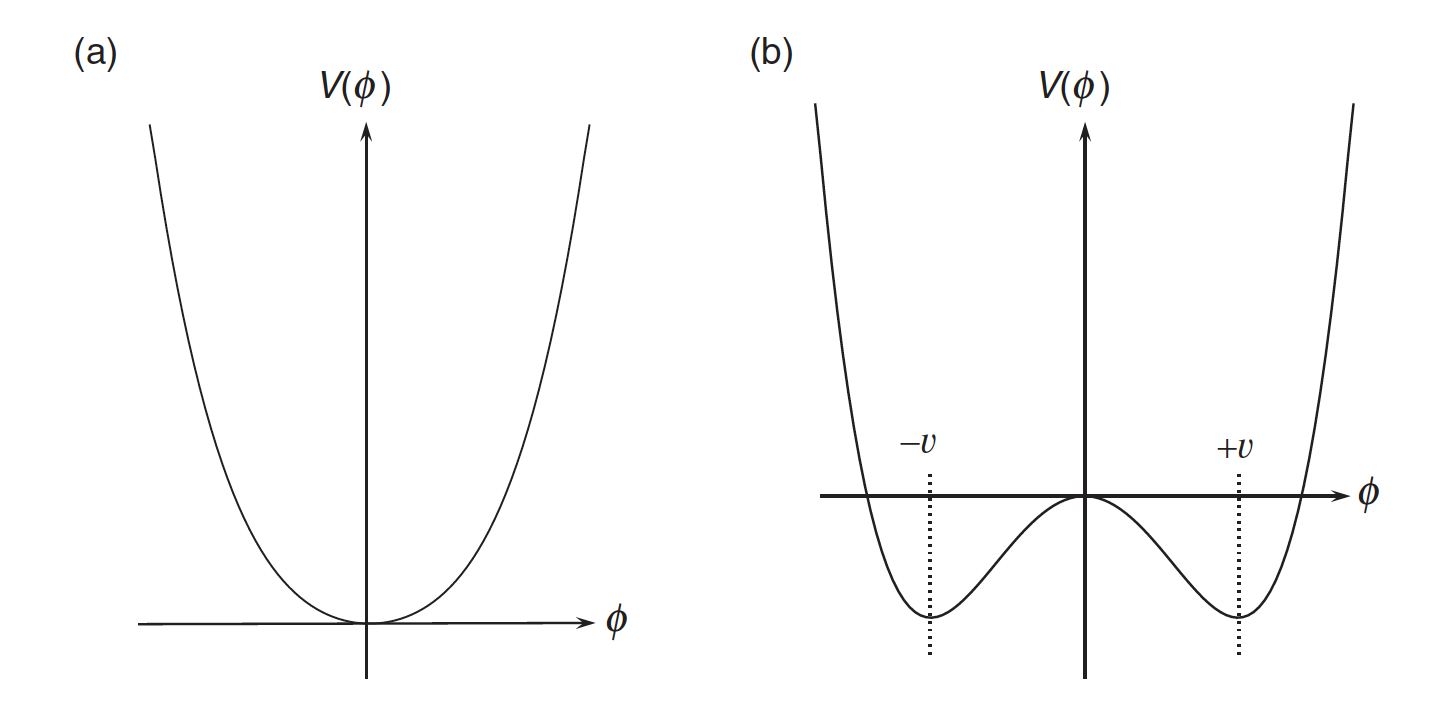
\includegraphics[width=0.55\textwidth]{Figures/c1/higgsPotential}
\caption{One dimensional rapresentation~\cite{} of the Higgs potential in case (a) of $\mu^2 > 0$ and minimum for $\phi = 0$ for an unbroken theory and in case (b) for $\mu^2 < 0$ and VEV for a spontaneous symmetry breaking.}
\label{fig:mexico}
\end{figure}

Starting from Eq.~\ref{eq:higgsM}, it can be written $\phi^+=\nicefrac{(\phi_1 + i\phi_2)}{\sqrt{2}}$ and $\phi^0=\nicefrac{(\phi_3 + i\phi_4)}{\sqrt{2}}$ and knowing $2\phi^\dag \phi = \phi^2_1+\phi^2_2+ \phi^2_3+ \phi^2_4 = v^2$ it is clear that the minima form a four-dimentional sphere.\\
Furthemore, studing the region of the vacuum and chosing a particular vacuum in the $SU(2)$ space with $\phi_3 = v$ and $\phi_1=\phi_2=\phi_4=0$, it is possible to expand around the minumum and write:
\begin{equation}
\label{eq:higgsphi2}
\phi(x) = \frac{1}{\sqrt{2}}\begin{pmatrix}
0\\
v+ H(x)
\end{pmatrix}
\end{equation}
where $H(x)$ is a scalar Higgs field. Now combining and replacing~\ref{eq:SMderivative} and~\ref{eq:higgsphi2} into the Lagrangian~\ref{eq:higgsL} it happens that photon field remains massless while the two mass terms for \PW and \PZ bosons appears:
\begin{align}
\left(\frac{vg_2}{2}\right) ^2W^{+\mu}W^-_{\mu} \; &\rightarrow \; m^2_W = \frac{g_2^2v^2}{4}\label{eq:massW}\\
\left(\frac{v\sqrt{g_1^2+g_2^2}}{2}\right)^2\frac{Z^{\mu}Z_{\mu}}{2} \; &\rightarrow \; m^2_Z = \frac{(g_1^2+g_2^2)v^2}{4}\label{eq:massZ}
\end{align}



\clearpage
\section{Beyond the Standard Model}\label{sec:bsm}
